\begin{figure*}[t]
\centering
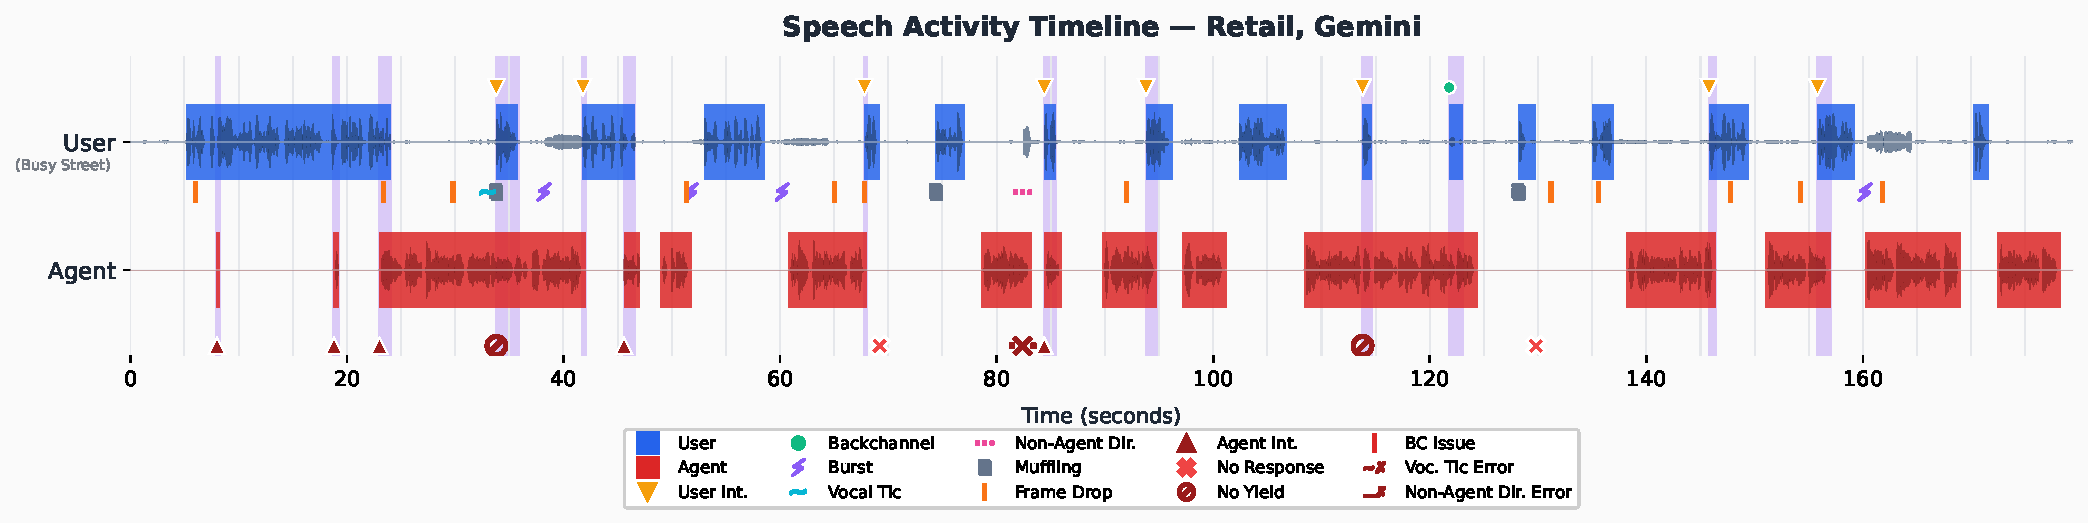
\includegraphics[width=\textwidth]{figures/task_41_data/speech activity timeline.pdf}
\caption{Speech activity timeline from a Retail domain simulation with \new{\texttt{gemini-live-2.5}}\old{Gemini Live}. A customer calls about exchanging a jigsaw puzzle and correcting their address. The legend distinguishes \textit{observations} (User Int.\ = user interruption, Non-Agent Dir.\ = speech to someone other than the agent, Burst = environmental burst noise) from \textit{evaluation markers} (Agent Int.\ = agent interruption, BC Issue = incorrect backchannel handling, Voc.\ Tic Error / Non-Agent Dir.\ Error = agent incorrectly yielding or responding to these stimuli).}
\label{fig:speech-timeline}
\end{figure*}

\paragraph{Timeline Walkthrough.}  Figure~\ref{fig:speech-timeline} illustrates our evaluation on a 3-minute Retail conversation with street noise. Key phenomena include: agent interruptions (red $\blacktriangle$) revealing turn-taking calibration; user interruptions where the agent yields but fails to respond (no-response error $\times$); non-agent-directed speech (pink \ldots) where the agent incorrectly yields; and backchannels (green $\circ$) correctly recognized as acknowledgment. Audio degradation (frame drops, muffling, burst noise) tests acoustic robustness throughout. This single example illustrates the density of phenomena our framework can simulate and measure: the audio signal contains 8 user interruptions, 12 frame drops, 3 background noise bursts, 3 muffling events, 1 vocal tic, 1 non-agent-directed speech, and 1 backchannel; from these, the evaluation identifies 5 agent interruptions, 2 no-response errors, and 1 vocal tic detection error (full transcript in Appendix~\ref{app:examples}).